%% !TEX root = manual.tex

\chapter{Clang Source-to-Source Auto-Skeletonization via Pragmas}
\label{clangTutorial}

There are three main examples of auto-skeletonization with pragmas in the \sstmacro source code in the \inlineshell{skeletons} directory.
These applications are Lulesh, HPCG, and CoMD.
The auto-skeletonizing compiler is designed to do three main things:

\begin{itemize}
\item Redirect global variable accesses to thread-specific values
\item Turn off large memory allocations that would prevent scalable simulation
\item Estimate time of compute-intensive kernels instead of executing them
\end{itemize}

\section{Pragma Overview}

\begin{figure}[h!]
\centering
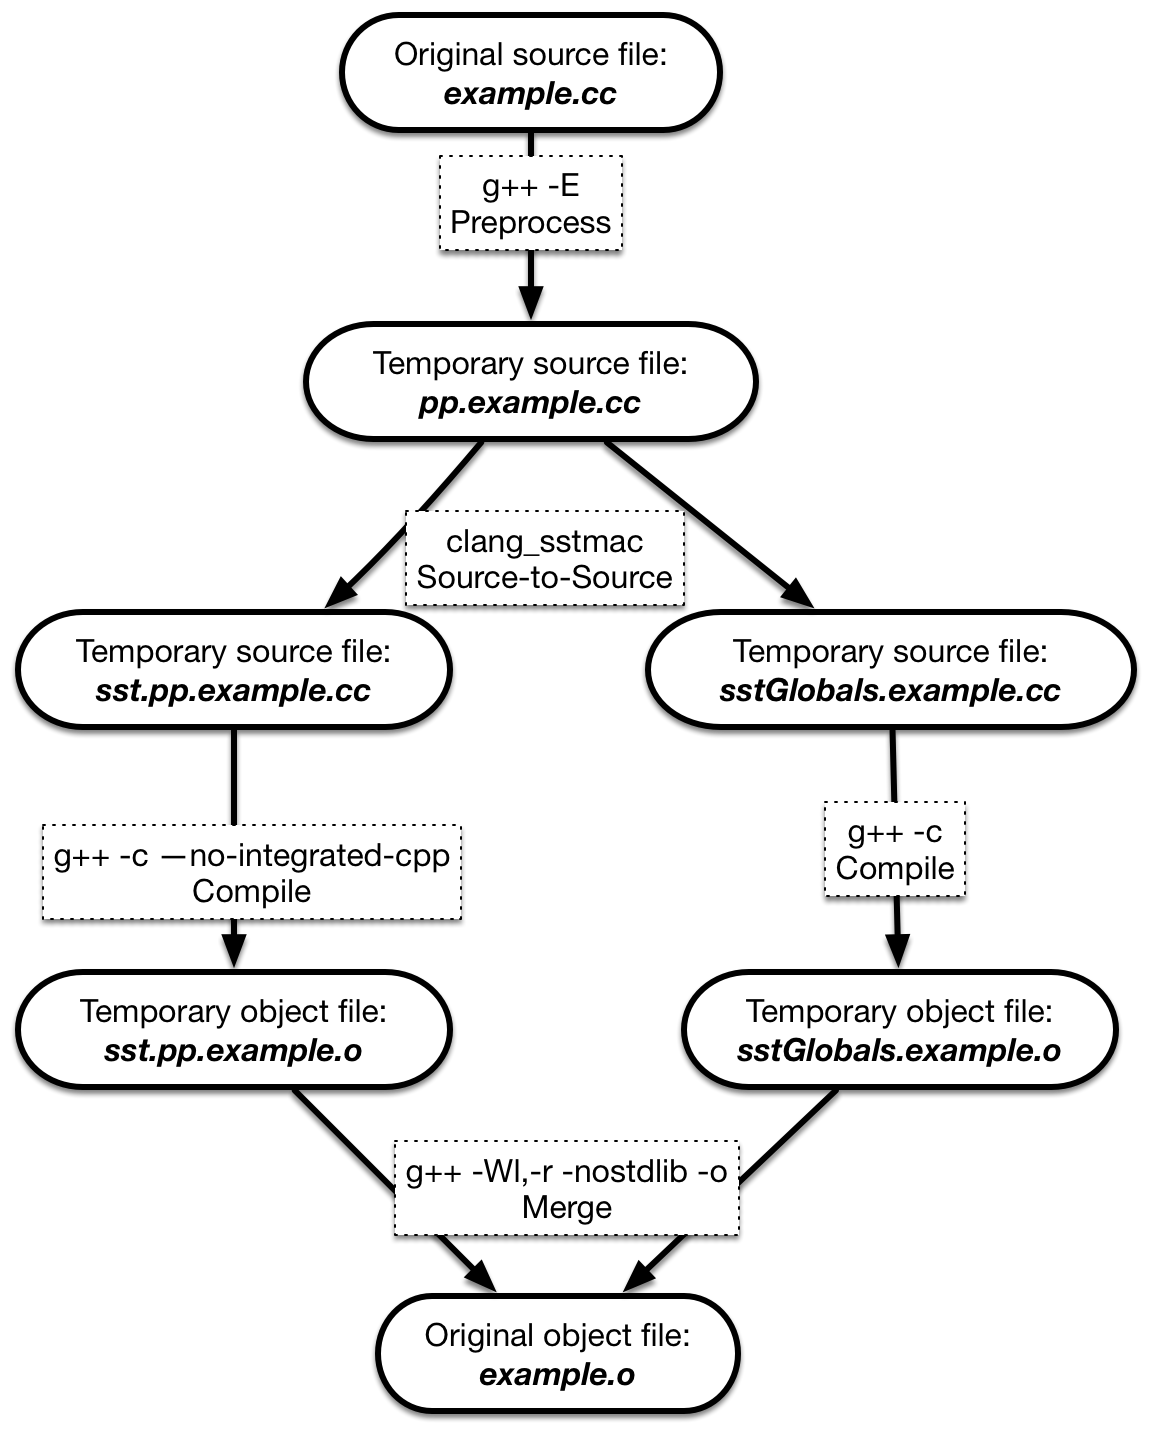
\includegraphics[width=0.66\textwidth]{figures/compilerWorkflow}
\caption{Source-to-source transformation workflow for SST compiler. For C source files, g++ can be swapped with gcc. The choice of underlying compiler is actually arbitrary and can be clang, gcc, icc, etc.}
\label{fig:compilerWorkflow}
\end{figure}

\subsection{Compiler workflow}
The source-to-source compiler operates on a pre-processed source file.
The source code transformation generates a temporary source file.
This temporary source file is then compiled into the target object file.
Global variables require static registration of C++ variables.
Here another temporary C++ source file (even if the original file is C)
is generated that has all static global variable registrations.
The corresponding object file is merged with the original object file,
creating a complete \sstmacro object file with the transformed code and C++ static registrations.
This workflow is shown in Figure \ref{fig:compilerWorkflow}.

\subsection{Compiler Environment Variables}

\subsubsection{SSTMAC\_SRC2SRC: Default 1}
If set to zero, deactivates the source-to-source transformation. 
The compiler wrapper will then compile the code into the simulator, but will not redirect any global variable accesses or perform any skeletonization.

\subsubsection{SSTMAC\_SKELETONIZE: Default 0}
If set to zero, deactivates skeletonization. 
This does not deactivate global variable redirection.
Thus, with \inlineshell{SSTMAC_SRC2SRC=1} and \inlineshell{SSTMAC_SKELETONIZE=0},
\sstmacro will act as an MPI emulator executing a full code but with global variables refactored to maintain correctness.

%\subsubsection{SSTMAC\_MEMOIZE: Default 0}
%If set to nonzero, activates memoization hooks. 
%This deactivates all global variable refactoring, all symbol interception, and all skeletonization.

\subsubsection{SSTMAC\_HEADERS: No default}
The compiler wrapper will only redirect global variables that it knows should definitely be modified.
All global variables found in source files will be redirected.
\inlinecode{extern} global variables found in header files are more difficult.
Certain system global variables like \inlinecode{stderr} should not be modified and so are left as global variable constants.
By default, global variables in a header file are NOT redirected unless explicitly specified in a header configuration file.
The variable \inlineshell{SSTMAC_HEADERS} should give the full path of a file containing the list of header files.
Header file paths in the file should be one per line and should be the full path, not a relative path.

\subsubsection{SSTMAC\_DELETE\_TEMPS: Default 1}
If non-zero, the compiler cleans up all temporary files. 
If you wish to keep temporary files to view them for debugging, set to zero.
All temporary, intermediate source files will otherwise be deleted at the end of compilation.

\section{Basic Replacement Pragmas}
When skeletonization is active (see \inlineshell{SSTMAC_SKELETONIZE}), these pragmas will cause replacements in the original source code.
Pragmas appy to the next statement in the source code.
For compound statements such as a for-loop with a multi-statement body, the pragma applies to the entire for-loop.
\subsection{pragma sst delete: no arguments}
This deletes the next statement from the source code.
If the statement declares a variable that is used later in the code, this will cause a compile error.
Consider an example from the Lulesh source code.

\begin{CppCode}
#pragma sst delete
    testnorms_data.values[i] = normr/normr0;
\end{CppCode}
In the skeleton, the residual is not actually computed and the \inlinecode{testnorms_data} array is not actually allocated.
Thus this statement should be deleted and not actually executed in the skeleton.

\subsection{pragma sst replace [to\_replace:string] [new\_text:C++ expression]}
This applies a string replace to a variable or function call in the next statement.
Consider an example from Lulesh.

\begin{CppCode}
#pragma sst replace volo 1
   deltatime() = (Real_t(.5)*cbrt(volo(0)))/sqrt(Real_t(2.0)*einit);
\end{CppCode}
The function call \inlinecode{volo(0)} is not valid in the skeleton since volumes are not actually computed.
Here we simply estimate that all cells have unit volume replacing \inlinecode{volo(0)} with \inlinecode{1}.

\subsection{pragma sst init [new\_value:string]}
This pragma can only apply to a binary equals operator assigning a value.
The pragma changes the right-hand side to use the given new value.
For example, in Lulesh:

\begin{CppCode}
#pragma sst init nullptr
  destAddr = &domain.commDataSend[pmsg * maxPlaneComm] ;
\end{CppCode}
The send buffer \inlinecode{domain.commDataSend} is not allocated in the skeleton and thus is not valid to use.
The pragma causes the skeleton to simply set \inlinecode{destAddr} to \inlinecode{nullptr}.

\subsection{pragma sst return [new\_value:C++ expression]}
Pragma is equivalent to \inlinecode{pragma sst init}. This replaces the target of a return statement with the given expression.
This produces a compiler error if applied to anything but a return statement.

\subsection{pragma sst keep}
During the skeletonization process, some transformations occur automatically even without pragmas. 
For example, all MPI calls have input buffers converted to null pointers to indicate a simulated MPI call.
If the MPI call should be emulated with real payloads, the MPI call must be explicitly marked with \inlinecode{pragma keep}.
An example can be found in the HPCG skeleton:

\begin{CppCode}
#pragma sst keep
  MPI_Allreduce(&localNumberOfNonzeros, &totalNumberOfNonzeros, ...)
\end{CppCode}
The actual allreduce operation is carried out, summing the the local number into the total number of nonzeroes.

\subsection{pragma sst keep\_if [condition:C++ bool expression]}
More control over whether transformations are skipped is provided by \inlinecode{keep_if}.
An example is found in CoMD.

\begin{CppCode}
#pragma sst keep_if count < 16
   MPI_Allreduce(sendBuf, recvBuf, count, MPI_DOUBLE, MPI_SUM, MPI_COMM_WORLD);
\end{CppCode}
Any small allreduce operations are kept. 
Any allreduce operations larger than a given cutoff are simulated without emulating the actual buffer operations.

\subsection{pragma sst empty}
This pragma is applied to functions. The function prototype is kept, but an empty body is inserted instead of the actual code.
This can be useful for deleting large blocks of computation inside a function.

\subsection{pragma sst branch\_predict [condition:C++ expression]}
The branch prediction pragma can be applied in two different contexts.
We will revisit the pragma in the context of compute skeletonization below.
The branch prediction pragma should only be applied to an if-statement.
Much like the replace pragmas, it swaps out the given if condition with a new expression.

The branch prediction pragmas become necessary when skeletonizing.
Certain values may not be computed or certain variables marked null.
If these values are then used in an if predicate,
the skeletonizing compiler cannot deduce the correct behavior for the application.
When an ambiguous predicate is found, the compiler will usually print a warning and just assume the predicate is false.
Predicates are often almost always true or almost always false. 
Thus most uses of this pragma will simply supply \inlinecode{true} or \inlinecode{false} as the replacement.
However, any arbitrary C++ boolean expression can be given as the replacement.
The new predicate expression (like the original), must not involve any null variables.

\section{Memory Allocation Pragmas}
\subsection{pragma sst malloc}
Applied to any statement in which the right-hand side is a malloc. This sets the left-hand side to \inlinecode{NULL}.
This is critical for turning off large memory allocations on data structures not required for control-flow.


\subsection{pragma sst new}
Applied to any statement in which the right-hand side a C++ operator new. This sets the left-hand side to \inlinecode{nullptr}.
This is critical for turning off large memory allocations on data structures not required for control-flow.

\section{Data-Driven Type Pragmas}
\subsection{pragma sst null\_variable}
This applies to variable declarations. If pragma is not applied to a declaration, a compiler error is given.
A null variable is one in which all operations involving the variable should be deleted.
This usually applies to large data arrays that should never be allocated and therefore never dereferenced.
An example can be seen in CoMD:

\begin{CppCode}
#pragma sst null_variable
   int* nAtoms;         //!< total number of atoms in each box
\end{CppCode}
The array is not allocated and all statements operating on the array are deleted.

This pragma is much more powerful than simply using \inlinecode{pragma sst new}.
\inlinecode{pragma sst new} simply turns off a given memory allocation setting it to a null value.
If the array is dereferenced later in code, this causes a segmentation fault.
By marking a declaration as null, the compiler can flag where segmentation faults would occur when running the skeleton.

In most cases, all operations involving the null variable are deleted.
However, there may be cases where the compiler may decide deleting an operation cannot be done automatically since
it may affect control flow, e.g., if the variable is used inside an if-statement.
When this occurs, a compiler error is thrown flagging where the ambiguity occurs.
Another pragma must then be applied to that statement to tell the compiler how to proceed.

\subsection{pragma sst null\_type [type alias] [list allowed functions]}
This applies to C++ class variable declarations. If pragma is not applied to a declaration, a compiler error is given.
This essentially works the same way as \inlinecode{null_variable}, but allows certain member functions to be kept instead of deleted.
Consider an example from Lulesh:

\begin{CppCode}
#pragma sst null_type sstmac::vector size resize empty
   std::vector<Real_t> m_x ;  /* coordinates */
\end{CppCode} 
Here we wish to indicate the vector is ``null'' and should not actually allocate memory or allow array accesses.
However, we still wish to track the vector size and whether it is empty.
The first argument to the pragma is a new type name that implements the ``alias'' functionality.
For \inlinecode{std::vector}, \sstmacro automatically provides the alias.
For illustration, that code is reproduced here:

\begin{CppCode}
namespace sstmac {
class vector {
 public:
  void resize(unsigned long sz){
    size_ = sz;
  }

  unsigned long size() const {
    return size_;
  }

  template <class... Args>
  void push_back(Args... args){
    ++size_;
  }

  template <class... Args>
  void emplace_back(Args... args){
    ++size_;
  }

  bool empty() const {
    return size_ == 0;
  }

 private:
  unsigned long  size_;
};
}
\end{CppCode}
This empty vector class allows the type to track its size, but not actually hold any data.
All places in the Lulesh code that an \inlinecode{std::vector} is used are substituted with the new type.

The remaining arguments to the pragma are the list of functions we wish to mark as valid.
In this case, even though the alias vector class provides more functions, we only allow \inlinecode{size}, \inlinecode{resize}, and \inlinecode{empty} to be called.



\section{Compute Pragmas}
\subsection{pragma sst compute and pragma omp parallel}
Compute-intensive should not be executed natively.
Instead, a compute model should be used to estimate the elapsed time.
Compute model replacements are automatically triggered by any OpenMP parallel pragmas.
The corresponding block or for-loop is not executed, instead calling out to a compute model to estimate time.
Currently, compute modeling is done via a very basic static analysis.
The static analysis attempts to count the number of integer and floating point operations.
It also estimates the number of memory reads and writes.
These four counters are passed to a coarse-grained processor model for time estimates.
For more details, see \inlinecode{sstmac_compute_detailed} in the source code.
Numerous examples can be found in the Lulesh, HPCG, and CoMD skeleton applications.

\subsection{pragma sst loop\_count [integer: C++ expression]}
If the \inlinecode{sst compute} or \inlinecode{omp parallel} pragma are applied to an outer loop with one or more inner loops,
the compute model static analysis might fail.
This occurs when the inner loop control flow depends on the actual execution.
Any variables declared \emph{inside} the compute block are not valid to use in the compute estimate since they will be skeletonized and deleted.
Only variables in scope at the beginning of the outer loop are safe to use in compute modeling.

When the static analysis fails, a corresponding compiler error is thrown.
This usually requires giving a loop count hint.
Consider the example from HPCG:

\begin{CppCode}
#pragma omp parallel for
  for (local_int_t i=0; i< localNumberOfRows; i++) {
    int cur_nnz = nonzerosInRow[i];
   #pragma sst loop_count 27
    for (int j=0; j<cur_nnz; j++) mtxIndL[i][j] = mtxIndG[i][j];
  }
\end{CppCode}
The static analysis fails on \inlinecode{cur_nnz}.
However, that value is almost always 27.
Thus we can safely tell the compiler to just assume the loop count is 27.

\subsection{pragma sst branch\_predict [float: C++ expression]}
Similar to the way that loop counts can break the static analysis, if statements inside a loop skeletonized with \inlinecode{omp parallel} or \inlinecode{sst compute} can also be problematic.
If the predicate depends on a variable declared \emph{inside} the skeletonzied block,
the static analysis will break since it cannot predict when and how often to assume true or false.
In contrast to the branch prediction pragma previously used, branch prediction pragmas inside a compute block must give a number between 0 and 1.
This can either be a literal float or expression that computes a float value.
Consider an example from CoMD:

\begin{CppCode}
#pragma sst branch_predict 0.2
  if(r2 <= rCut2 && r2 > 0.0){
\end{CppCode}
Inside the compute block, a compute may or may not occur depending on whether a particle distance is less than a cutoff.
Based on the way CoMD constructs unit cells and halo regions, running CoMD shows that about 1 in 5 neighbor interactions are actually below the cutoff.
Thus we given the branch prediction the hint 0.2.

\subsection{pragma sst advance\_time [units] [time to advance by]}
This pragma advances the simulator time by the specified amounts of time. It can be placed before any statement. The units can be the following: sec, msec, usec or nsec for Seconds, milliseconds, microseconds and nanoseconds respectively. 

%% !TEX root = manual.tex

\section{Memoization pragmas}\label{sec:memoization}

\subsection{Memoization models}
To understand the memoization pragmas, we first introduce how models get constructed in the SST/macro runtime.
Source-to-source transformations based on the pragmas causes the following hooks to get inserted:

\begin{CppCode}
int sstmac_startMemoize(const char* token, const char* model);
void sstmac_finish_memoize0(int tag, const char* token);
void sstmac_finish_memoize1(int tag, const char* token, double p1);
void sstmac_finish_memoize2(int tag, const char* token, double p1, double p2);
...
\end{CppCode}
A start call begins a memoization region for a specific name.
The start function must return an integer tag identifying the memoization instance.
This tag gets passed back into the finish function above.
This is primarily useful for thread-safe collection, but can be generally more useful.
The finish functions take input parameters. 
Given input parameters $x$,$y$ causes a function $F(x,y)$ to be fit to the timer or performance counters.

If building a skeleton application that uses memoization data, a different hook gets inserted:
\begin{CppCode}
void sstmac_compute_memoize0(const char* token);
void sstmac_compute_memoize1(const char* token, double p1);
void sstmac_compute_memoize2(const char* token, double p1, double p2);
...
\end{CppCode}
Assuming a model $F(x,y)$ has been fit in a memoization pass,
that function is invoked with the given parameters to estimate a time or performance counter.

Memoization models are implemented by inheriting from a standard class

\begin{CppCode}
struct RegressionModel {
...
virtual double compute(int n_params, const double params[], ImplicitState* state) = 0;
virtual int StartCollection() = 0;
virtual void finishCollection(int n_params, const double params[], ImplicitState* state) = 0;
...
\end{CppCode}
A call to \inlinecode{sstmac_finish_memoize2} causes \inlinecode{finishCollection(2,..)} to get invoked on the model.
The \inlinecode{states} object is discussed more later in \ref{subsec:implicitStates}.
For now, \inlinecode{compute} only returns a double (total time).
Generalized performance models are planned for future versions.
Models are registered using the SST/macro factory system. 
If wanting to add a least-squares model, factory register as:

\begin{CppCode}
struct least_squares : public regression model {
 FactoryRegister("least_squares", OperatingSystem::RegressionModel, least_squares)
\end{CppCode}

\subsection{pragma sst memoize [skeletonize(...)] [model(...)] [inputs(...)] [name(...)]}
\begin{itemize}
\item skeletonize: boolean for whether code block should still be executed or remove entirely (default: true)
\item model: string name for a type of model (e.g. linear, kmeans) specifying which model to construct and fit (no default)
\item inputs: a comma-separated list of C++ expressions that are the numeric inputs
\item name: a unique name to use for identifying the memoization region (default: see below)
\end{itemize}
If the \inlinecode{name} parameter is not given, the file and line number is used for basic expressions while the function name is used if applied to a function.
Consider the example:

\begin{CppCode}
#pragma sst memoize skeletonize(true) model(least_squares) inputs(ncol,nlink,nrow) 
void dgemm(int ncol, int nlink, int nrow, double* left, double* right);
\end{CppCode}
When running the memoization pass, the memoization hooks get invoked as:

\begin{CppCode}
int tag = sstmac_startMemoize("dgemm", "least_squares");
dgemm(....);
sstmac_finish_memoize3(tag, "dgemm", ncol, nlink, nrow);
\end{CppCode}
With \inlinecode{skeletonize} set to true, the skeleton app would be:

\begin{CppCode}
sstmac_computeMemoize("dgemm", ncol, nlink, nrow);
\end{CppCode}
With skeletonize set to false:

\begin{CppCode}
sstmac_computeMemoize("dgemm", ncol, nlink, nrow);
dgemm(...);
\end{CppCode}
Both the memoization function and the original function would both get invoked.

\subsection{pragma sst implicit\_state X(Y) ...}\label{subsec:implicitStates}
The implicit state pragma sets certain hardware or software states not captured by the inputs to the memoization pragma.
This might involve DVFS states, different runs of a task in which data is ``cold'' or ``hot'' in cache, or different types of cores.
The implicit state lasts for the scope of the statement:

\begin{CppCode}
#pragma sst implict_state ...
{
 //all statements here have that state
}

#pragma sst ImplicitState ...
fxn(...) //implicit state lasts the entire function
\end{CppCode}

The arguments to the pragma are best understood by example:

\begin{CppCode}
#pragma sst ImplicitState dvfs(1) cache(hot)
fxn(...)
\end{CppCode}
This causes a source code transformation to:

\begin{CppCode}
sstmac_set_ImplicitState2(dvfs,1,cache,hot);
fxn(...);
sstmac_unset_ImplicitState2(dvfs,cache);
\end{CppCode}
For now, the functions take integer arguments (this may get relaxed to arbitrary strings).
Thus, e.g. enums must be available or compilation will fail:

\begin{CppCode}
enum states {
 dvfs=0,
 cache=1
};
enum cache_states {
 cold=0,
 hot=1
};
\end{CppCode}

If a \inlinecode{sstmac_finish_memoize} function got invoked, the states could be read.
The class \inlinecode{ImplicitState} is a base class only and carries no data by default.
Specific memoization models are intended to be used only with known implicit state classes.
As such, the memoization model \inlinecode{collect}, etc, functions must dynamic cast to an expected type.
A library of standard implicit state implementations is planned for future releases.

